\documentclass[9pt,technote,a4paper]{IEEEtran}
\usepackage[utf8]{inputenc}
\usepackage[T1]{fontenc}
\usepackage[portuguese]{babel}
\usepackage{csquotes}
\usepackage{amsmath,amssymb,amsfonts}
\usepackage{graphicx}
\usepackage{booktabs}
\usepackage{algorithm}
\usepackage{algpseudocode}
\usepackage{xcolor}
\usepackage{tikz}
\usetikzlibrary{arrows.meta,positioning,fit,backgrounds}
\usepackage{hyperref}

\hypersetup{
    colorlinks=true,
    linkcolor=blue!50!black,
    citecolor=blue!50!black,
    urlcolor=blue!50!black
}

\floatname{algorithm}{Algoritmo}
\algrenewcommand\algorithmicrequire{\textbf{Entrada:}}
\algrenewcommand\algorithmicensure{\textbf{Saída:}}

% Controle dos blocos TODO (troque para \showtodosfalse na versão final)
\newif\ifshowtodos
\showtodostrue

\newcommand{\todo}[2][TODO]{%
    \ifshowtodos
    \par\vspace{4pt}%
    \noindent\colorbox{amberbg}{%
        \parbox{\dimexpr\linewidth-2\fboxsep\relax}{%
            \footnotesize\textbf{\textcolor{amberfg}{[#1]}} #2%
        }%
    }%
    \par\vspace{4pt}%
    \fi
}
\definecolor{amberbg}{RGB}{255,248,225}
\definecolor{amberfg}{RGB}{153,77,0}

\title{Reconhecimento de Locutor em Conjunto Aberto Embarcado em ESP32-S3 via GMM-UBM, Normalização Cepstral e Filtro de Wiener Casado à Voz}

\author{
    \IEEEauthorblockN{Projeto RecVoz --- Grupo de Processamento Digital de Sinais e Sistemas Embarcados}
    \IEEEauthorblockA{Arquitetura de Borda em Microcontrolador ESP32-S3 (\texttt{hardware/recvoz-esp})}
}

\begin{document}
\maketitle

\todo[TODO 0 --- Metadados e Autoria]{%
    (1) Substituir \texttt{\textbackslash author} pelos nomes reais dos autores, departamento, instituição e e-mails.
    (2) Ao finalizar todos os itens abaixo, alterar \texttt{\textbackslash showtodostrue} para \texttt{\textbackslash showtodosfalse} no preâmbulo e recompilar.
}

\begin{abstract}
Este trabalho apresenta a modelagem matemática, a implementação embarcada e a validação experimental de um sistema de identificação de locutores em conjunto aberto (\textit{open-set}) operando integralmente em um microcontrolador ESP32-S3 sem PSRAM externa ($\approx 181\text{ KiB}$ de RAM dinâmica disponível), com amostragem a $16\text{ kHz}$ via microfone MEMS I2S INMP441. Partindo do diagnóstico quantitativo das falhas de um classificador clássico baseado na média temporal de coeficientes MFCC e $k$-NN cosseno --- nomeadamente contaminação por ruído estacionário durante o cadastro ao vivo (\textit{online enrollment}), deslocamento da inclinação espectral ($c_1$) entre sessões e disparos espúrios por energia subsônica ($< 80\text{ Hz}$) ---, propõe-se um \textit{pipeline} integrado por: (i) detector de atividade vocal (VAD) passa-banda ($80\text{--}7920\text{ Hz}$) com limiar adaptativo por relação sinal-ruído ($\mathrm{SNR} \ge +6\text{ dB}$); (ii) \textbf{filtro de Wiener espectral casado ao espectro médio da voz humana} ($\alpha = 0{,}8$, piso $-13\text{ dB}$, \textit{prior} vocal de $513$ bins em Flash) com banco de $40$ filtros na escala \textbf{Mel HTK} ($17$ coeficientes cepstrais $c_0\dots c_{16}$), calibração inicial no \textit{boot}, \textit{holdoff} de $2{,}5\text{ s}$ e guarda de estacionariedade; (iii) veto de ruído por âncora cepstral e energia de modulação articulatória ($\mathrm{mod}$); e (iv) modelo probabilístico \textbf{GMM-UBM} diagonal ($M = 8$ componentes, $D = 32$ dimensões em $c_1\dots c_{16}$ e $\Delta c_1\dots \Delta c_{16}$) com seleção de quadros ativos (\textit{Frame-VAD}, top $70\%$ em $c_0$), Normalização da Média Cepstral seletiva em $c_1$ (\textbf{CMN-$c_1$}) e adaptação MAP (\textit{Maximum A Posteriori}) incremental de passo único na placa. Os experimentos em conjunto fechado atingem $100\%$ de acurácia em todas as $10$ partições de sessão, consumindo apenas $1024\text{ bytes}$ na NVS por locutor cadastrado e $348{,}8\text{ KiB}$ de binário final ($66\%$ da partição livre). Em avaliação \textit{open-set} com $6$ locutores gravados no INMP441 ($19$ sessões, $102$ janelas), o UBM externo (\textit{Google FLEURS PT-BR}, $44\,100$ quadros) acoplado ao filtro de Wiener casado à voz, banco Mel HTK ($40$ filtros, $17$ MFCCs) e \textit{Frame-VAD} atinge \textbf{AUC-ROC de $\mathbf{95{,}5 \pm 2{,}7\%}$}, \textbf{EER de $\mathbf{9{,}4 \pm 6{,}0\%}$} e \textbf{FAR de $\mathbf{6{,}8 \pm 5{,}3\%}$}, superando amplamente Centroide ($81{,}7\%$ AUC, $24{,}6\%$ EER), $k$-NN ($79{,}2\%$ AUC, $31{,}8\%$ EER), SVM-RBF ($69{,}1\%$ AUC, $35{,}6\%$ EER) e GMM independente ($66{,}2\%$ AUC, $40{,}7\%$ EER), ocupando $2{,}19\text{ KiB}$ para o UBM e $2{,}0\text{ KiB}$ para o \textit{prior} vocal em Flash.
\end{abstract}

\begin{IEEEkeywords}
Reconhecimento de locutor, GMM-UBM, normalização da média cepstral (CMN), filtro de Wiener casado à voz, sistemas embarcados, ESP32-S3.
\end{IEEEkeywords}

\section{Introdução}
\label{sec:intro}

A identificação automática de locutores em dispositivos de borda (\textit{edge audio}) impõe um compromisso severo entre robustez acústica e orçamento computacional. Em ambientes reais, o sinal captado sofre degradação simultânea por ruído aditivo estacionário (ventiladores, sistemas HVAC, zumbido de rede elétrica de $60\text{ Hz}$) e por distorções convolutivas decorrentes da resposta impulsiva do recinto, da distância ao microfone e da resposta em frequência do transdutor~\cite{reynolds2000,furui1981,rabiner1993}.

Em cenários de operação em \textbf{conjunto aberto} (\textit{open-set}) com \textbf{cadastro ao vivo} de novos usuários (denominados aqui locutor visitante $S_v$), o problema agrava-se: caso o detector de atividade vocal (VAD) ou o extrator de características não isole adequadamente a voz humana do piso acústico da sala, o modelo matriculado passa a incorporar a assinatura espectral do próprio ambiente, gerando falsos positivos sempre que o ruído de fundo é capturado.

Na arquitetura inicial do sistema analisado, baseada em vetores médios de coeficientes cepstrais na escala Mel (MFCC) classificados por $k$-NN com distância cosseno, identificaram-se três limitações estruturais:
\begin{enumerate}
    \item \textbf{Vulnerabilidade do VAD a energia sub-$80\text{ Hz}$:} a medição de RMS sobre o sinal bruto permitia que oscilações graves ($11\text{--}80\text{ Hz}$) disparassem janelas silenciosas. Em uma das sessões de referência, $29$ de $70$ blocos ($41\%$) aceitos pelo VAD bruto possuíam energia vocal real na faixa de $80\text{--}7920\text{ Hz}$ de apenas $40\text{--}73$.
    \item \textbf{Dominância do coeficiente $c_1$ (inclinação espectral):} na média temporal de $c_1\dots c_{12}$, o coeficiente $c_1$ concentra aproximadamente $85\%$ da norma $L_2$ do vetor ($\approx 123{,}4$ contra $5\text{--}40$ nos demais coeficientes). Variações de sala ou posicionamento deslocaram $c_1$ ao vivo para $97{,}3$, induzindo inversões de ranking entre o locutor $S_1$ e o locutor $S_2$.
    \item \textbf{Colapso das derivadas temporais e inviabilidade de CMN:} a média temporal com sinal sobre $\Delta c_d$ e $\Delta^2 c_d$ tende a zero pela propriedade telescópica das diferenças finitas, inutilizando $26$ das $39$ dimensões. Além disso, a Normalização da Média Cepstral (CMN) não pode preceder uma média única global, pois anularia o próprio vetor de entrada do classificador.
\end{enumerate}

Para superar tais gargalos dentro dos limites de memória do ESP32-S3 ($\approx 181\text{ KiB}$ de RAM livre, sem PSRAM), este artigo formula e valida a substituição do $k$-NN por um classificador \textbf{GMM-UBM + CMN}, acoplado a um \textit{front-end} de condicionamento passa-banda, supressão espectral controlada e veto por modulação articulatória (Figura~\ref{fig:arquitetura}).

\subsection{Trabalhos Relacionados}
\label{sec:related}

A evolução do reconhecimento de locutor independente de texto percorreu três paradigmas principais: modelos generativos de misturas Gaussianas com modelo universal de fundo (GMM-UBM)~\cite{reynolds1995,reynolds2000}, análise de fatores em espaço total (\textit{i-vectors})~\cite{dehak2011} e representações profundas extraídas por redes neurais temporais, como \textit{x-vectors}~\cite{snyder2018} e ECAPA-TDNN~\cite{desplanques2020}. Embora arquiteturas neurais dominem \textit{benchmarks} em servidores, seus requisitos típicos --- milhões de parâmetros, dezenas de megabytes de ativações e latência elevada sem acelerador matricial --- extrapolam o orçamento de microcontroladores de borda sem PSRAM externa~\cite{warden2019}.

Em contrapartida, o GMM-UBM com covariâncias diagonais e adaptação MAP restrita às médias~\cite{reynolds2000} apresenta propriedades particularmente favoráveis a sistemas embarcados: (i) baixo custo de inferência em ponto flutuante ($O(M \cdot T \cdot D)$); (ii) cadastro ao vivo determinístico em uma única passagem sobre poucos segundos de fala, sem retropropagação; e (iii) armazenamento compacto em memória não volátil ($M \times D$ floats por locutor). Combinado à CMN~\cite{furui1981} e à filtragem espectral de Wiener casada ao perfil médio da fala~\cite{loizou2013}, o modelo oferece um ponto de operação atraente entre robustez acústica e viabilidade em hardware restrito.

\begin{figure*}[t]
    \centering
    \begin{tikzpicture}[
        node distance=5mm and 5.5mm,
        block/.style={
            rectangle, draw=black!75, fill=blue!5, rounded corners=2pt,
            minimum height=8.5mm, text width=21mm, align=center, font=\scriptsize
        },
        ctrl/.style={
            rectangle, draw=black!75, fill=orange!10, rounded corners=2pt,
            minimum height=8.5mm, text width=21mm, align=center, font=\scriptsize
        },
        outblk/.style={
            rectangle, draw=black!75, fill=green!8, rounded corners=2pt,
            minimum height=8.5mm, text width=21mm, align=center, font=\scriptsize
        },
        arr/.style={-{Stealth[length=2mm]}, semithick}
    ]
        \node[block] (mic) {INMP441\\I2S 16 kHz};
        \node[block, right=of mic] (bp) {DC Blocker +\\Butterworth BP};
        \node[block, right=of bp] (vad) {VAD Adaptativo\\($\mathrm{SNR} \ge +6$ dB)};
        \node[block, right=of vad] (stft) {STFT + Wiener\\Casado à Voz};
        \node[block, right=of stft] (mfcc) {Mel HTK (40)\\17c + $\Delta, \Delta^2$};
        \node[ctrl, right=of mfcc] (veto) {Veto de Ruído\\($\mathrm{mod}$ + âncora)};

        \node[block, below=7mm of veto] (cmn) {Frame-VAD (70\%)\\+ CMN-$c_1$ ($D{=}32$)};
        \node[block, left=14mm of cmn] (gmm) {GMM-UBM\\($M=8$, LLR)};
        \node[outblk, left=14mm of gmm] (out) {Decisão ($\tau$) +\\OLED / Serial};

        \node[ctrl, below=6mm of cmn] (map) {Adaptação MAP\\(\texttt{enroll}, $r=8$)};
        \node[outblk, left=14mm of map] (nvs) {Persistência NVS\\(1024 B/locutor)};

        \draw[arr] (mic) -- (bp);
        \draw[arr] (bp) -- (vad);
        \draw[arr] (vad) -- (stft);
        \draw[arr] (stft) -- (mfcc);
        \draw[arr] (mfcc) -- (veto);
        \draw[arr] (veto) -- node[right, font=\tiny] {fala válida} (cmn);
        \draw[arr] (cmn) -- node[above, font=\tiny] {inferência} (gmm);
        \draw[arr] (gmm) -- (out);
        \draw[arr] (cmn) -- node[right, font=\tiny] {modo \texttt{enroll}} (map);
        \draw[arr] (map) -- (nvs);
        \draw[arr] (nvs) -- node[right, font=\tiny] {modelos} (gmm);
    \end{tikzpicture}
    \caption{Arquitetura de processamento do sistema embarcado RecVoz no ESP32-S3, integrando condicionamento passa-banda, VAD adaptativo, supressão espectral controlada, veto de ruído estacionário e classificação/matrícula GMM-UBM + CMN.}
    \label{fig:arquitetura}
\end{figure*}

\section{Aquisição, Condicionamento e VAD Adaptativo}
\label{sec:vad}

\subsection{Amostragem I2S e Filtragem Passa-Banda}
O microfone digital MEMS INMP441 é lido a $f_s = 16\,000\text{ Hz}$ por interface I2S ($24\text{ bits}$ úteis em palavras de $32\text{ bits}$). Inicialmente, aplica-se um filtro bloqueador DC de primeira ordem com $\alpha_{\mathrm{dc}} = 0{,}9957$ (corte em $\approx 10{,}9\text{ Hz}$):
\begin{equation}
    y_{\mathrm{dc}}[n] = x[n] - x[n-1] + \alpha_{\mathrm{dc}}\, y_{\mathrm{dc}}[n-1].
\end{equation}

Para rejeitar energia subsônica ($< 80\text{ Hz}$) e componentes próximas a Nyquist, o sinal normalizado passa por um filtro Butterworth passa-banda de $5^\text{a}$ ordem ($80\text{--}7920\text{ Hz}$) decomposto em cinco seções biquadráticas (SOS) aplicadas em dupla passada (\textit{zero-phase forward-backward}, \texttt{filtfilt}):
\begin{equation}
    H_{\mathrm{bp}}(z) = \prod_{k=1}^{5} \frac{b_{k,0} + b_{k,1} z^{-1} + b_{k,2} z^{-2}}{1 + a_{k,1} z^{-1} + a_{k,2} z^{-2}}.
\end{equation}

\subsection{VAD Passa-Banda e Limiar Adaptativo por SNR}
Em cada bloco de $100\text{ ms}$ ($N_b = 1600$ amostras), o RMS é computado exclusivamente após o estágio passa-banda:
\begin{equation}
    \mathrm{RMS}_{\mathrm{voz}}(b) = \sqrt{\frac{1}{N_b}\sum_{n=0}^{N_b-1} \left(32768 \cdot x_{\mathrm{bp}}[n]\right)^2}.
\end{equation}
Quando o perfil de ruído estacionário encontra-se calibrado com nível $\mathrm{RMS}_{\text{ruído}}$, o limiar efetivo de disparo do VAD adapta-se para impor margem mínima de $+6\text{ dB}$ de SNR:
\begin{equation}
    \mathrm{VAD}_{\mathrm{efetivo}} = \max\!\left(\mathrm{VAD}_{\mathrm{base}},\; 2 \cdot \mathrm{RMS}_{\text{ruído}}\right).
\end{equation}
A Figura~\ref{fig:vad_esp} ilustra o comportamento do VAD sobre uma captura real de $3\text{ s}$ no ESP32-S3, isolando os $20$ blocos vocais ($2{,}0\text{ s}$) acima do limiar $\mathrm{VAD}_{\mathrm{base}} = 300$ e descartando os intervalos de silêncio e pausas.

\begin{figure}[t]
    \centering
    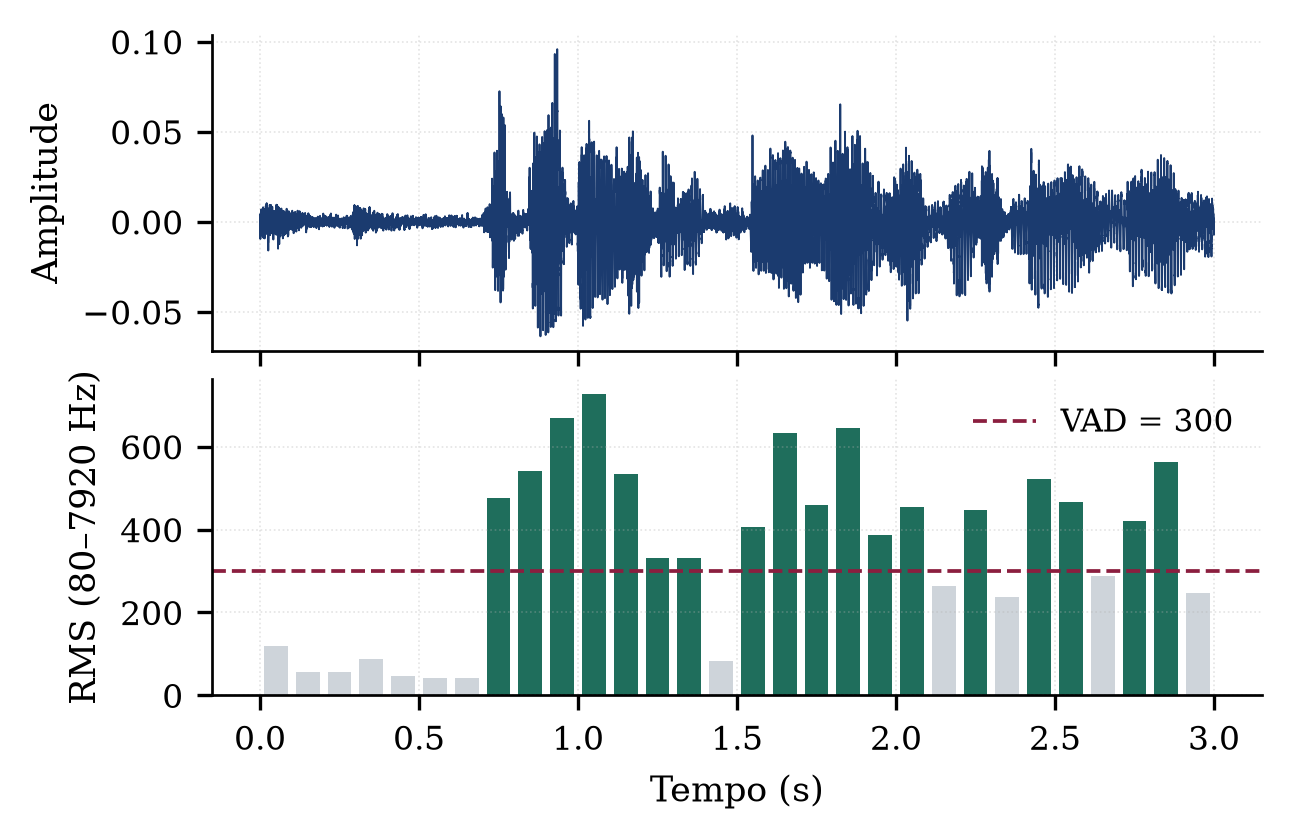
\includegraphics[width=\columnwidth]{figs/fig_vad_esp.png}
    \caption{Captura real de $3\text{ s}$ no INMP441 do ESP32-S3. Topo: forma de onda normalizada. Base: RMS na banda de $80\text{--}7920\text{ Hz}$ por bloco de $100\text{ ms}$ (verde: aceitos; cinza: descartados).}
    \label{fig:vad_esp}
\end{figure}

\section{Extração MFCC e Supressão Espectral Segura}
\label{sec:mfcc}

\subsection{Espectrograma Mel e Coeficientes Dinâmicos}
Cada janela ativa de $2\text{ s}$ ($32\,000$ amostras) é segmentada por STFT com janela de Hann periódica $h[n] = 0{,}5 - 0{,}5\cos(2\pi n / N_{\mathrm{FFT}})$ de $N_{\mathrm{FFT}} = 1024$ amostras ($64\text{ ms}$), salto $H = 256$ amostras ($16\text{ ms}$) e preenchimento centrado por zeros, produzindo $T = 1 + \lfloor 32000/256 \rfloor = 126$ quadros. A densidade espectral de potência $P[t, k] = |X[t, k]|^2$ ($k = 0\dots 512$) sofre filtragem de Wiener casada à voz e é integrada por um banco de $M_{\mathrm{mel}} = 40$ filtros triangulares na escala \textbf{Mel HTK}:
\begin{equation}
    \mathrm{mel}_{\mathrm{HTK}}(f) = 2595 \log_{10}\!\left(1 + \frac{f}{700}\right),
\end{equation}
com energia por banda $E_{\mathrm{mel}}[t, m] = \sum_{k=0}^{512} W_{\mathrm{mel}}[m, k]\, \hat{P}[t, k]$ armazenada em formato esparso. Diferentemente da escala de Slaney (linear abaixo de $1\text{ kHz}$), a escala HTK é logarítmica desde $0\text{ Hz}$, concentrando maior resolução espectral na faixa de $80\text{--}1000\text{ Hz}$ (frequência fundamental $F_0$ e primeiro formante $F_1$), enquanto $40$ filtros suavizam harmônicos isolados e reduzem em $\approx 3\times$ a matriz DCT em Flash.

Após compressão logarítmica $L_0[t,m] = 10\log_{10}(\max(E_{\mathrm{mel}}[t,m], 10^{-10}))$ e piso dinâmico de $80\text{ dB}$ relativo ao pico de cada quadro ($L[t,m] = \max(L_0[t,m], \max_{m'} L_0[t,m'] - 80)$), aplica-se a DCT-II ortonormal ($17$ coeficientes estáticos $c_0\dots c_{16}$, preservando quefrencias superiores $c_{13}\dots c_{16}$ ligadas à anatomia do trato vocal que o corte clássico de ASR em $c_{12}$ descarta):
\begin{equation}
    c_n[t] = \sqrt{\frac{2-\delta_{n,0}}{M_{\mathrm{mel}}}} \sum_{m=0}^{M_{\mathrm{mel}}-1} L[t, m] \cos\!\left(\frac{\pi n (2m+1)}{2 M_{\mathrm{mel}}}\right).
\end{equation}
Para viabilizar execução em tempo real no ESP32-S3, a matriz $17 \times 40$ dos cossenos é pré-computada em Flash (\texttt{MFCC\_DCT}), eliminando chamadas a \texttt{cos()} em dupla precisão emulada. As derivadas de primeira ($\Delta$) e segunda ($\Delta^2$) ordens são obtidas por convolução com filtros de Savitzky-Golay de largura $9$ pontos ($w_1[i] = i/60$ para $i \in \{-4\dots 4\}$ e $w_2$ quadrático simétrico, com replicação das janelas de borda nos $4$ quadros extremos), compondo a matriz $M \in \mathbb{R}^{51 \times 126}$.

\subsection{Filtro de Wiener Casado ao Espectro de Voz e Veto de Ruído}
O espectro médio de ruído estacionário $\hat{N}[k]$ é estimado em lotes de $8192$ amostras ($0{,}512\text{ s}$, $33$ quadros). Como a potência instantânea de ruído gaussiano em cada bin $k$ segue uma distribuição exponencial ($\sigma = \mu$), calibrações sucessivas são integradas por média móvel exponencial ($\beta = 0{,}3$) e filtradas por um núcleo de suavização de $3$ pontos em frequência ($[0{,}25;\; 0{,}5;\; 0{,}25]$).

Para suprimir ruído estacionário sem distorcer os formantes vocais nem introduzir artefatos metálicos (\textit{musical noise}), aplica-se quadro a quadro um \textbf{filtro de Wiener espectral casado ao espectro médio da voz humana}~\cite{loizou2013}. Um \textit{prior} espectral normalizado $\bar{S}_{\mathrm{voz}}[k]$ ($\sum_{k=0}^{512}\bar{S}_{\mathrm{voz}}[k] = 1$, pico em $375\text{ Hz}$) é pré-estimado sobre $44\,100$ quadros do corpus \textit{Google FLEURS PT-BR}~\cite{conneau2023} e armazenado em Flash ($513$ floats, $2{,}0\text{ KiB}$). Em cada quadro $t$, estima-se a energia vocal excedente $E_{\mathrm{voz}}[t] = \max\!\big(\sum_k P[t,k] - \sum_k \hat{N}[k],\; 0{,}05\sum_k \hat{N}[k]\big)$ e calcula-se o ganho suave de Wiener por bin:
\begin{equation}
    H[t, k] = \max\!\left(\frac{E_{\mathrm{voz}}[t]\,\bar{S}_{\mathrm{voz}}[k]}{E_{\mathrm{voz}}[t]\,\bar{S}_{\mathrm{voz}}[k] + \alpha\,\hat{N}[k]},\; \sqrt{f_{\mathrm{piso}}}\right),
\end{equation}
\begin{equation}
    \hat{P}[t, k] = H[t, k]^2\, P[t, k],
\end{equation}
com $\alpha = 0{,}8$ e piso proporcional $f_{\mathrm{piso}} = 0{,}05$ ($-13\text{ dB}$). Quando $\sum_k \hat{N}[k] = 0$, o filtro reduz-se a \textit{pass-through} exato. A Figura~\ref{fig:noise_suppression} ilustra a atenuação do piso de ruído nos domínios FFT e Mel.

\begin{figure}[t]
    \centering
    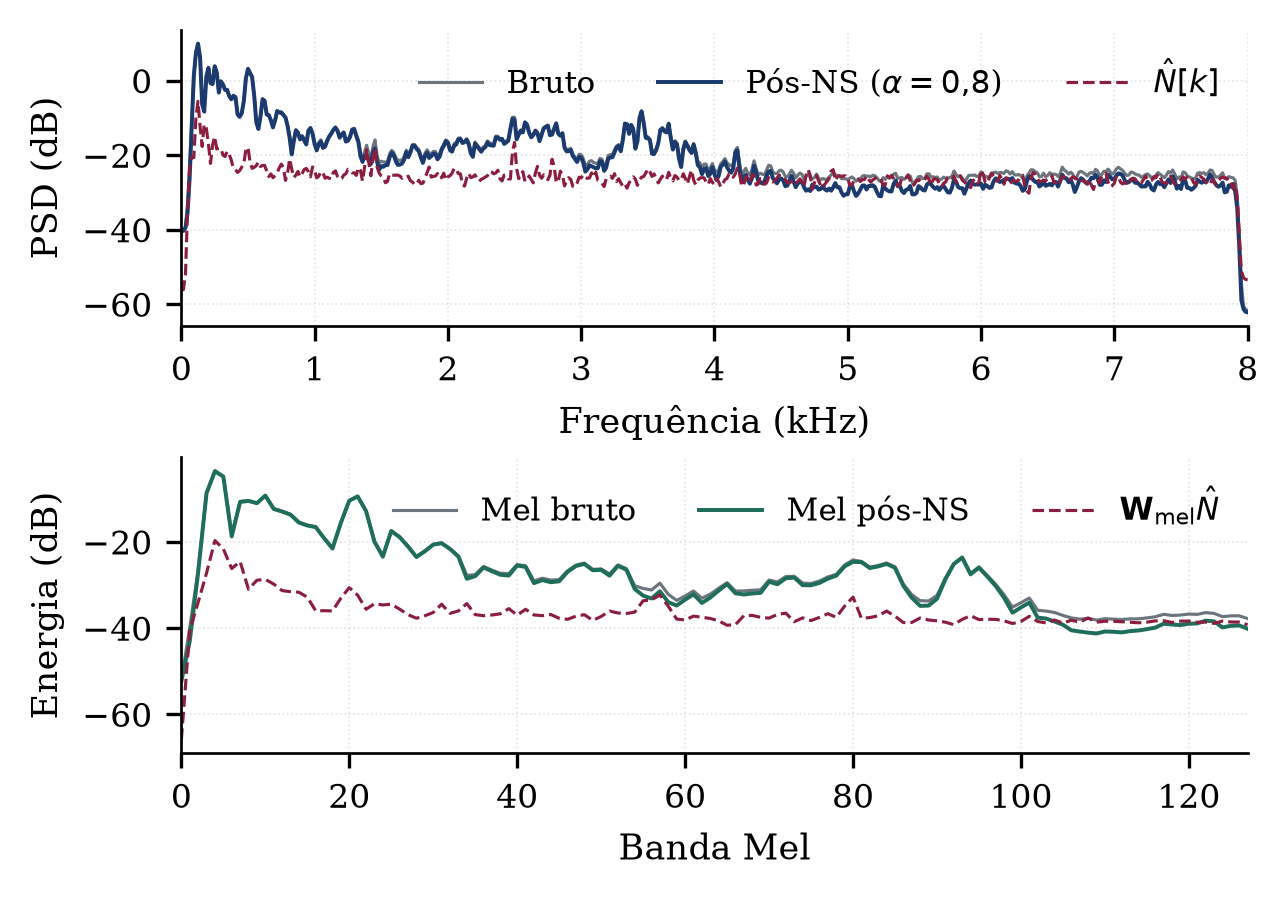
\includegraphics[width=\columnwidth]{figs/fig_noise_suppression.png}
    \caption{Efeito da supressão espectral sobre fala capturada no ESP32-S3 com ruído estacionário ($\alpha = 0{,}8$, $f_{\mathrm{piso}} = 0{,}05$). Topo: PSD nos $513$ bins FFT. Base: energia integrada nas $128$ bandas Mel.}
    \label{fig:noise_suppression}
\end{figure}

Para evitar a contaminação do perfil $\hat{N}[k]$ por sílabas iniciais antes do disparo de voz e vetar ruídos estacionários que ultrapassem o VAD, implementa-se o Algoritmo~\ref{alg:ns_veto}, baseado na âncora cepstral $\mathbf{a}_{\text{ruído}}$ e na energia de modulação articulatória:
\begin{equation}
    \mathrm{mod}(M) = 5{,}0 \sqrt{\sum_{d=14}^{25} \left(\frac{1}{T}\sum_{t=0}^{T-1} M[d, t]^2\right)}.
\end{equation}
A Figura~\ref{fig:modulacao} evidencia a separação entre ruído estacionário ($26{,}8\text{--}28{,}3$) e janelas de fala ($51{,}2\text{--}82{,}2$) frente ao limiar $\mathrm{mod}_{\min} = 32{,}0$.

\begin{figure}[t]
    \centering
    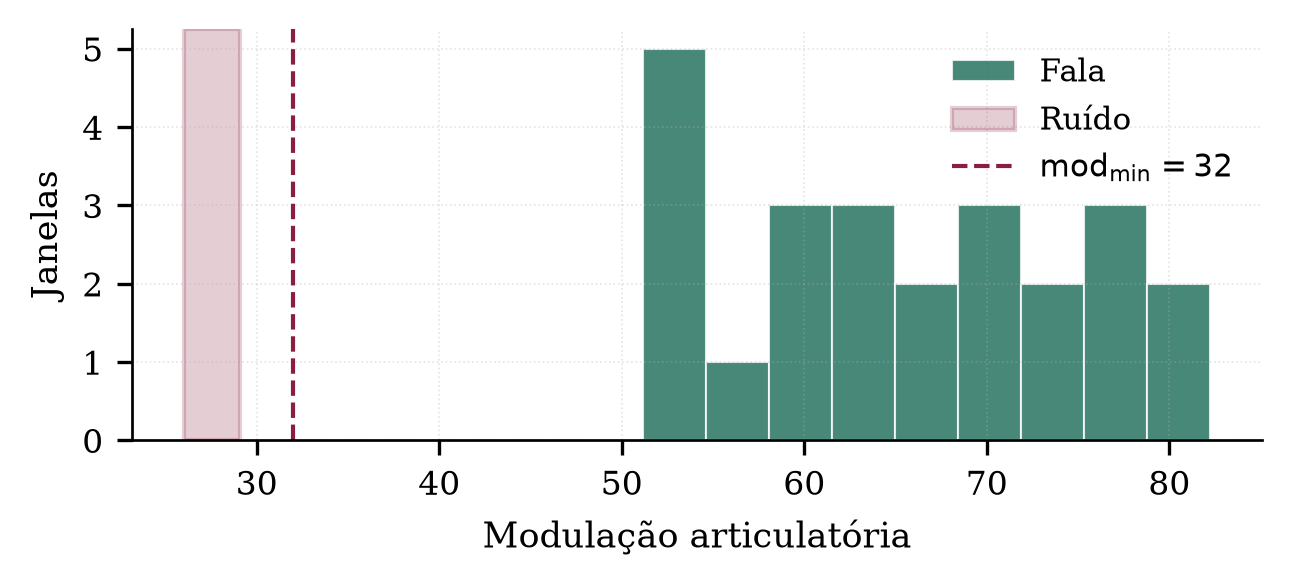
\includegraphics[width=\columnwidth]{figs/fig_modulacao.png}
    \caption{Separação entre ruído estacionário e fala humana pela energia de modulação articulatória ($\mathrm{mod}$) calculada sobre $\Delta c_1\dots \Delta c_{12}$.}
    \label{fig:modulacao}
\end{figure}

\begin{algorithm}[t]
\caption{Calibração Segura e Veto de Ruído Estacionário}
\label{alg:ns_veto}
\begin{algorithmic}[1]
\Require Bloco de entrada $b$ ($1600$ amostras), janela capturada $W$ ($32000$ amostras)
\Ensure Perfil $\hat{N}[k]$, âncora $\mathbf{a}_{\text{ruído}}$, decisão de veto booleana
\If{boot inicial}
    \State Ler $8192$ amostras $\rightarrow$ inicializar $\hat{N}[k]$, $\mathbf{a}_{\text{ruído}}$ e $\mathrm{RMS}_{\text{ruído}}$
\EndIf
\If{$\mathrm{RMS}_{\mathrm{voz}}(b) > \mathrm{VAD}_{\mathrm{efetivo}}$}
    \State Zerar acumulador de silêncio e contador de \textit{holdoff} ($s_{\mathrm{fill}} \leftarrow 0$)
\ElsIf{$\mathrm{RMS}_{\mathrm{voz}}(b) \le \frac{2}{3}\mathrm{VAD}_{\mathrm{efetivo}}$ por $25$ blocos contínuos ($2{,}5\text{ s}$)}
    \State Acumular $8192$ amostras $\rightarrow$ calcular $\mathrm{mod}_{\mathrm{cal}}$
    \If{$\mathrm{mod}_{\mathrm{cal}} < 26{,}0$} \Comment{Garante ausência de fala infiltrada}
        \State Atualizar $\hat{N}[k]$ via EMA ($\beta=0{,}3$) + suavização $[0{,}25, 0{,}5, 0{,}25]$
        \State Atualizar $\mathbf{a}_{\text{ruído}}$ e $\mathrm{RMS}_{\text{ruído}}$
    \EndIf
\EndIf
\State Extrair $M \in \mathbb{R}^{39\times 126}$ de $W$; calcular $\mathrm{mod}(M)$ e $d_{\mathrm{ns}} = 1 - \cos(\bar{\mathbf{m}}_{1:38}, \mathbf{a}_{1:38})$
\If{$\mathrm{mod}(M) < \mathrm{mod}_{\min}$ \textbf{ou} ($\mathrm{mod}(M) < 48{,}0$ \textbf{e} $d_{\mathrm{ns}} \le d_{\min}$)}
    \State \Return \textbf{Veto}: \texttt{RUIDO AMBIENTE}
\EndIf
\end{algorithmic}
\end{algorithm}

\section{Modelagem GMM-UBM com CMN por Janela}
\label{sec:gmm}

\subsection{Análise do Viés Cepstral e Justificativa do Modelo}
A Figura~\ref{fig:mfcc_fisher} expõe o motivo pelo qual a distância cosseno sobre médias MFCC é frágil sob mudança de canal. Os coeficientes $c_2$ e $c_6$ apresentam elevado poder discriminante entre $S_1$ e $S_2$ (escores de Fisher de $2{,}95$ e $2{,}67$), enquanto $c_1$ exibe baixo escore ($0{,}59$) aliado à maior amplitude absoluta ($123{,}4$). Na captura ao vivo no ESP32-S3, $c_1$ caiu para $97{,}3$, dominando a métrica cosseno.

\begin{figure}[t]
    \centering
    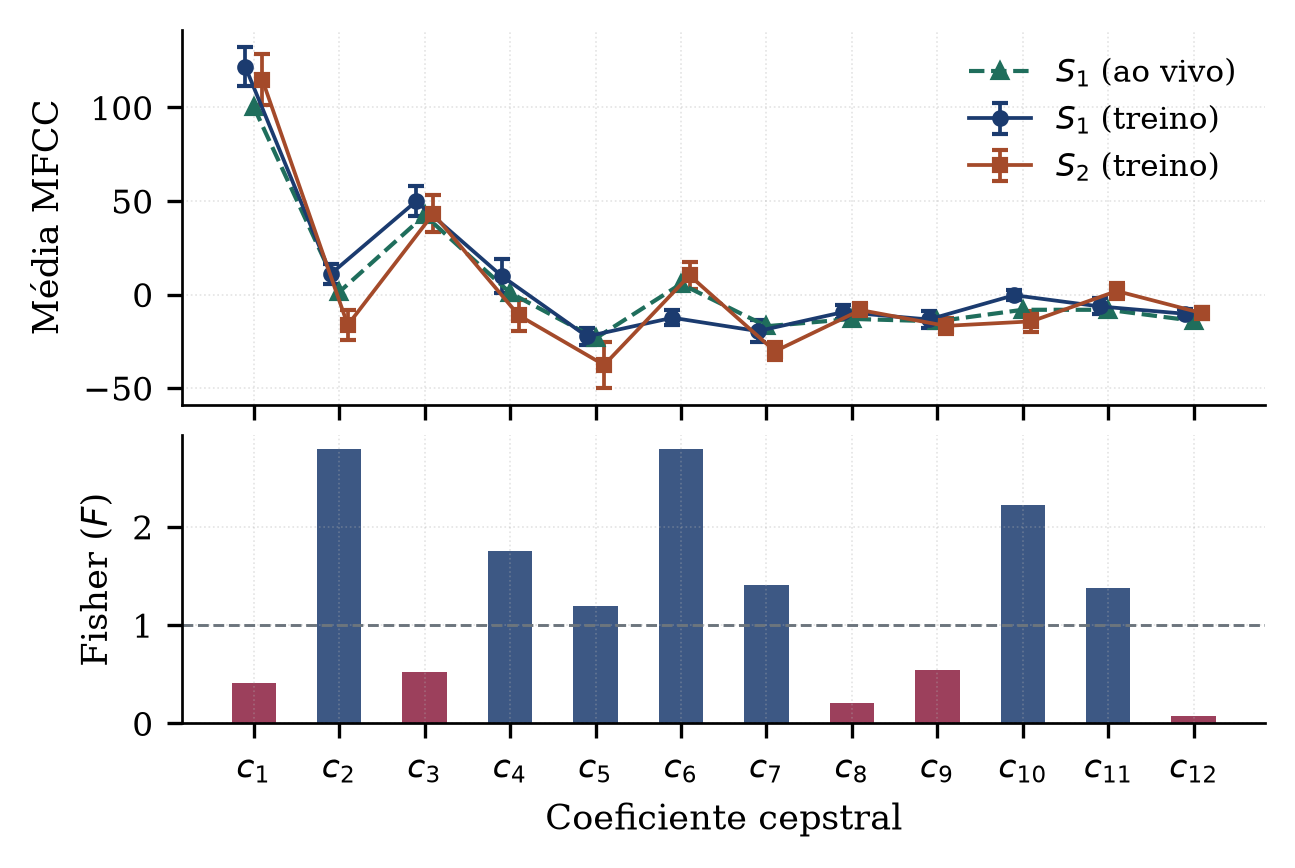
\includegraphics[width=\columnwidth]{figs/fig_mfcc_fisher.png}
    \caption{Topo: perfil médio de $c_1\dots c_{12}$ para $S_1$ e $S_2$ (treino) e $S_1$ (ESP32 ao vivo), evidenciando o deslocamento de canal em $c_1$. Base: escore de Fisher por coeficiente.}
    \label{fig:mfcc_fisher}
\end{figure}

\subsection{Seleção de Quadros Ativos, Normalização CMN-$c_1$ e Adaptação MAP}
Antes da classificação, aplica-se um \textbf{VAD em nível de quadro (\textit{Frame-VAD})} selecionando os $70\%$ quadros de maior energia logarítmica $c_0[t]$ ($T' = 88$ quadros ativos por janela de $2\text{ s}$), descartando micropausas articulatórias e consoantes surdas que diluem o LLR e contaminam as estatísticas da janela --- reduzindo simultaneamente em $30\%$ o custo computacional do GMM-UBM. Ao operar quadro a quadro no subespaço de $D = 32$ dimensões $\mathbf{x}_t = [c_1[t]\dots c_{16}[t],\; \Delta c_1[t]\dots \Delta c_{16}[t]]^\top$ (excluindo $c_0$ e $\Delta c_0$ para manter invariância ao ganho), aplica-se a \textbf{CMN seletiva em $c_1$} sobre os $T'$ quadros ativos ($\tilde{x}_{t,1} = x_{t,1} - \frac{1}{T'}\sum_{\tau} x_{\tau,1}$), cancelando o viés dominante de inclinação espectral/canal sem apagar a assinatura anatômica do trato vocal em $c_2\dots c_{16}$. A distribuição universal de fala é representada por um UBM diagonal com $M = 8$ Gaussianas:
\begin{equation}
    p(\tilde{\mathbf{x}}_t \mid \lambda_{\mathrm{UBM}}) = \sum_{m=1}^{M} w_m\, \mathcal{N}(\tilde{\mathbf{x}}_t \mid \boldsymbol{\mu}_m^{\mathrm{UBM}},\, \boldsymbol{\Sigma}_m).
\end{equation}

Para execução eficiente em precisão simples (\texttt{float32}) no ESP32-S3, pré-computa-se em Flash a constante logarítmica de cada componente $C_m = -\frac{1}{2}\sum_{d=1}^{D}\ln(2\pi \sigma_{m,d}^2)$ e o inverso das variâncias $\Sigma_{m,d}^{-1}$. A log-verossimilhança parcial da componente $m$ no quadro $t$ resume-se a:
\begin{equation}
    \ell_{t, m}(\lambda) = \ln w_m + C_m - \frac{1}{2}\sum_{d=1}^{D} \left(\tilde{x}_{t,d} - \mu_{m,d}\right)^2 \Sigma_{m,d}^{-1},
\end{equation}
agregada com estabilidade via identidade \textit{log-sum-exp} ($\ell_t^* = \max_m \ell_{t,m}$):
\begin{equation}
    \log p(\tilde{\mathbf{x}}_t \mid \lambda) = \ell_t^* + \ln\!\left(\sum_{m=1}^{M} \exp(\ell_{t,m} - \ell_t^*)\right),
\end{equation}
prevenindo \textit{underflow} numérico em exponenciais de alta dimensão.

Na matrícula de um locutor $s$ (incluindo o cadastro ao vivo de $S_v$ em $7$ janelas de $2\text{ s}$), adaptam-se apenas as médias via MAP com fator de relevância $r = 8{,}0$ (Algoritmo~\ref{alg:gmm_ubm}), requerendo exatamente $M \times D = 192$ floats ($768\text{ bytes}$) por locutor na NVS. Estudos de sensibilidade sobre $M \in \{8, 12, 16, 32\}$ e entre CMN e CMVN indicaram que $M = 8$ com CMN (sem escalamento de variância) evita \textit{overfitting} nos conjuntos de matrícula curtos ($15\text{ s}$) e atinge $100\%$ ($23/23$) em \textit{Window-LOO} com margem mínima de $+0{,}127$ (contra $22/23$ em $M=12, 16$ e $18/23$ em $M=32$). Na inferência, decide-se pelo maior \textit{Log-Likelihood Ratio} médio:
\begin{equation}
    \mathrm{LLR}(s) = \frac{1}{T}\sum_{t=1}^{T}\Big[\log p(\tilde{\mathbf{x}}_t \mid \lambda_s) - \log p(\tilde{\mathbf{x}}_t \mid \lambda_{\mathrm{UBM}})\Big],
\end{equation}
mapeado para compatibilidade de interface em $d_{\mathrm{eq}}(s) = \mathrm{clip}((1 - \mathrm{LLR}(s))/2,\; 0,\; 1)$, onde o limiar padrão $\tau = 0{,}42$ corresponde a exigir $\mathrm{LLR} \ge +0{,}16$.

\begin{algorithm}[t]
\caption{Adaptação MAP Incremental e Inferência GMM-UBM}
\label{alg:gmm_ubm}
\begin{algorithmic}[1]
\Require Parâmetros UBM $\{w_m, \boldsymbol{\mu}_m^{\mathrm{UBM}}, \boldsymbol{\Sigma}_m^{-1}\}_{m=1}^M$, janelas de entrada
\Ensure Modelo adaptado $\{\hat{\boldsymbol{\mu}}_m^{(s)}\}$ ou locutor vencedor
\Procedure{EnrollMAP}{janelas $W_1 \dots W_K$}
    \State $N_m \leftarrow 0,\; \mathbf{S}_m \leftarrow \mathbf{0} \quad \forall m \in \{1\dots M\}$
    \For{$k = 1 \dots K$}
        \State Extrair $\mathbf{X}^{(k)} \in \mathbb{R}^{T\times 24}$ e aplicar CMN $\rightarrow \tilde{\mathbf{X}}^{(k)}$
        \For{$t = 1 \dots T$}
            \State $\gamma_m \leftarrow \frac{w_m \mathcal{N}(\tilde{\mathbf{x}}_t \mid \boldsymbol{\mu}_m^{\mathrm{UBM}}, \boldsymbol{\Sigma}_m)}{\sum_j w_j \mathcal{N}(\tilde{\mathbf{x}}_t \mid \boldsymbol{\mu}_j^{\mathrm{UBM}}, \boldsymbol{\Sigma}_j)}$
            \State $N_m \leftarrow N_m + \gamma_m$; \quad $\mathbf{S}_m \leftarrow \mathbf{S}_m + \gamma_m \tilde{\mathbf{x}}_t$
        \EndFor
    \EndFor
    \State $\alpha_m \leftarrow \frac{N_m}{N_m + r}$; \quad $\hat{\boldsymbol{\mu}}_m^{(s)} \leftarrow \alpha_m \frac{\mathbf{S}_m}{N_m} + (1 - \alpha_m)\boldsymbol{\mu}_m^{\mathrm{UBM}}$
\EndProcedure
\Procedure{ClassifyWindow}{janela $W$, modelos $\{\lambda_s\}$}
    \State Aplicar CMN em $W \rightarrow \tilde{\mathbf{X}}$; \quad $L_{\mathrm{ubm}} \leftarrow \frac{1}{T}\sum_t \log p(\tilde{\mathbf{x}}_t \mid \lambda_{\mathrm{UBM}})$
    \For{cada locutor ativo $s$}
        \State $\mathrm{LLR}(s) \leftarrow \frac{1}{T}\sum_t \log p(\tilde{\mathbf{x}}_t \mid \lambda_s) - L_{\mathrm{ubm}}$
    \EndFor
    \State $s^* \leftarrow \arg\max_s \mathrm{LLR}(s)$; \quad $d_{\mathrm{eq}} \leftarrow \mathrm{clip}((1-\mathrm{LLR}(s^*))/2, 0, 1)$
    \State \Return $(d_{\mathrm{eq}} \le \tau)\; ?\; s^* : \texttt{DESCONHECIDO}$
\EndProcedure
\end{algorithmic}
\end{algorithm}

\section{Arquitetura Embarcada, Persistência e Orçamento Computacional}
\label{sec:firmware}

\subsection{Integração no Firmware, Memória e Persistência NVS}
O firmware é estruturado em módulos desacoplados sob FreeRTOS: \texttt{audio\_in} (leitura contínua I2S DMA), \texttt{capture} (VAD passa-banda e agrupamento de $20$ blocos de $100\text{ ms}$), \texttt{mfcc} (processamento DSP de $40$ bandas Mel e filtro de Wiener casado à voz), \texttt{gmm\_ubm} (componente portátil de inferência GMM-UBM, \textit{Frame-VAD}, CMN-$c_1$ e adaptação MAP), \texttt{speaker\_db} (gerenciamento de locutores e persistência NVS) e \texttt{recvoz\_display} (interface OLED SSD1306 via I2C). Para evitar transbordamento de pilha (\textit{stack overflow}) durante a extração de características na tarefa principal, os vetores intermediários de quadro (\texttt{power[513]}, \texttt{mel[40]}) e os buffers de janela (\texttt{s\_win} com $64\text{ KiB}$ e \texttt{s\_m} com $\approx 20\text{ KiB}$) são alocados estaticamente, e a \textit{stack} da tarefa \texttt{main} foi dimensionada em $8192\text{ bytes}$.

A persistência em NVS (\textit{Non-Volatile Storage}) utiliza versionamento explícito de limiar (\texttt{tauver = 4}) para migrar automaticamente instalações anteriores para $\tau = 0{,}70$ ($d_{\mathrm{eq}} = \mathrm{clip}(1 - \mathrm{LLR}/5, 0, 1)$, exigindo $\mathrm{LLR} \ge +1{,}50$). Cada locutor extra matriculado ao vivo ocupa um \textit{slot} contendo nome (\texttt{x\%dn}), vetores médios legados (\texttt{x\%dv}), médias GMM-UBM adaptadas (\texttt{x\%dg}, $768\text{ bytes}$) e máscara de sobrescrita de fábrica (\texttt{ovr}), permitindo substituir um locutor de fábrica pelo seu perfil gravado diretamente no microfone local sem perda de reversibilidade (\texttt{reset}).

\subsection{Complexidade e Consumo de Recursos no ESP32-S3}
A Tabela~\ref{tab:recursos} detalha o orçamento estático do GMM-UBM + CMN na CPU do ESP32-S3 ($160\text{ MHz}$). O UBM completo ocupa apenas $1{,}66\text{ KiB}$ em memória flash (\texttt{const}), enquanto a pontuação de um locutor sobre $126$ quadros requer $M \cdot T \cdot D = 24\,192$ operações de diferença quadrática ponderada. Para evitar pico duplo de alocação no \textit{heap} interno, o filtro passa-banda \texttt{filtfilt} opera \textit{in-place} com bordas espelhadas de $33$ amostras na pilha ($264\text{ B}$), economizando $128\text{ KiB}$ de RAM dinâmica. A Tabela~\ref{tab:latencia} apresenta o perfil real de latência e memória medido diretamente na placa via comando serial \texttt{bench 20} (\texttt{esp\_timer\_get\_time}, $N=20$ janelas, $3$ locutores ativos e supressão espectral ligada): a inferência completa pós-captura leva $961{,}8 \pm 17{,}1\text{ ms}$ ($< 1\text{ s}$), preservando $44{,}4\text{ KiB}$ de \textit{heap} livre mínimo e $3{,}95\text{ KiB}$ de margem na pilha de $8\text{ KiB}$ da tarefa principal.

\begin{table}[t]
\centering
\footnotesize
\setlength{\tabcolsep}{3.5pt}
\caption{Orçamento de memória e complexidade por locutor no ESP32-S3.}
\label{tab:recursos}
\begin{tabular}{lcc}
\toprule
\textbf{Componente} & \textbf{MFCC + $k$-NN} & \textbf{GMM-UBM + CMN} \\
\midrule
Modelo de fundo + \textit{prior} (Flash) & --- & $2{,}19 + 2{,}00\text{ KiB}$ \\
NVS / locutor & $1428\text{ B}$ ($7{\times}51$) & $1024\text{ B}$ ($8{\times}32$) \\
Operações / locutor & $k$-NN ($30{\times}50$) & $22\,528$ MACs ($88$ q.) \\
Binário (\texttt{recvoz-esp.bin}) & $345{,}8\text{ KiB}$ & $348{,}8\text{ KiB}$ ($66\%$ livre) \\
\bottomrule
\end{tabular}
\end{table}

\begin{table}[t]
\centering
\scriptsize
\setlength{\tabcolsep}{3pt}
\caption{Perfil real de latência e memória medido no ESP32-S3 ($160\text{ MHz}$, média $\pm$ DP em $N=20$ janelas, $3$ locutores, NS ativo).}
\label{tab:latencia}
\begin{tabular}{lc}
\toprule
\textbf{Estágio / Métrica} & \textbf{Valor Medido} \\
\midrule
Filtro passa-banda (\texttt{filtfilt} \textit{in-place}, $32\,000$ am.) & $101{,}6 \pm 1{,}6\text{ ms}$ \\
STFT + Wiener Voz + Mel + DCT + $\Delta/\Delta^2$ & $491{,}3 \pm 17{,}5\text{ ms}$ \\
CMN + inferência GMM-UBM (por locutor) & $121{,}0 \pm 1{,}0\text{ ms}$ \\
CMN + inferência GMM-UBM ($3$ locutores) & $363{,}0 \pm 2{,}9\text{ ms}$ \\
Adaptação MAP (\texttt{enroll}, $7$ janelas) & $1024{,}6 \pm 17{,}7\text{ ms}$ \\
Latência total fim a fim (pós-captura) & $961{,}8 \pm 17{,}1\text{ ms}$ \\
\textit{Heap} livre em repouso / mínimo no pico & $192{,}5\text{ KiB}$ / $44{,}4\text{ KiB}$ \\
Margem livre na \textit{stack} \texttt{main} ($8\text{ KiB}$) & $3{,}95\text{ KiB}$ ($4040\text{ B}$) \\
\bottomrule
\end{tabular}
\end{table}

\section{Resultados Experimentais}
\label{sec:resultados}

\subsection{Validação Offline em Conjunto Fechado e Estudo de Ablação}
A Tabela~\ref{tab:comparacao} e a Figura~\ref{fig:gmm_llr} comparam os classificadores na base de validação inicial ($23$ janelas: $9$ de $S_1$ e $14$ de $S_2$) e na captura ao vivo do ESP32-S3. Todas as $7$ suítes C (\texttt{knn}, \texttt{gmm}, \texttt{mfcc}, \texttt{ns}, \texttt{commands}, \texttt{audio}, \texttt{persistence}) e os $9$ testes Python atingiram $100\%$ de aprovação. A Tabela~\ref{tab:ablacao} organiza o estudo de ablação sobre número de componentes $M$, normalização cepstral, supressão espectral e uso de derivadas temporais.

\begin{table}[t]
\centering
\footnotesize
\setlength{\tabcolsep}{3.5pt}
\caption{Desempenho comparativo: média MFCC + $k$-NN vs. GMM-UBM + CMN.}
\label{tab:comparacao}
\begin{tabular}{lcc}
\toprule
\textbf{Critério} & \textbf{MFCC + $k$-NN} & \textbf{GMM-UBM + CMN} \\
\midrule
\textit{Window-LOO} & $23/23$ ($100\%$) & $23/23$ ($100\%$) \\
\textit{Holdout} por sessão & $9/9$ ($100\%$) & $9/9$ ($100\%$) \\
\texttt{fixture} ($S_1$ vs.\ $S_2$) & $\Delta d = +0{,}021$ & $\Delta \mathrm{LLR} = +1{,}298$ \\
ESP32 ao vivo ($S_1$) & $d$: $0{,}022$ vs.\ $0{,}027$ & $\mathrm{LLR}$: $+0{,}350$ vs.\ $-0{,}576$ \\
\bottomrule
\end{tabular}
\end{table}

\begin{table}[t]
\centering
\scriptsize
\setlength{\tabcolsep}{2.6pt}
\caption{Estudo de ablação do GMM-UBM interno em conjunto aberto (seed 42; $10$ janelas conhecidas e $34$ de impostores inéditos, banco Mel 40 + \textit{Frame-VAD} 70\%).}
\label{tab:ablacao}
\begin{tabular}{lcccc}
\toprule
\textbf{Configuração} & \textbf{Acc} & \textbf{FAR} & \textbf{FRR} & \textbf{EER} \\
\midrule
$M{=}8$, CMN, $c{+}\Delta$, Wiener Voz & $100\%$ & $35{,}3\%$ & $50{,}0\%$ & $40{,}6\%$ \\
$M{=}4$, CMN, $c{+}\Delta$, Wiener Voz & $100\%$ & $32{,}4\%$ & $50{,}0\%$ & $52{,}9\%$ \\
$M{=}12$, CMN, $c{+}\Delta$, Wiener Voz & $90{,}0\%$ & $44{,}1\%$ & $40{,}0\%$ & $40{,}6\%$ \\
$M{=}16$, CMN, $c{+}\Delta$, Wiener Voz & $100\%$ & $35{,}3\%$ & $50{,}0\%$ & $34{,}1\%$ \\
$M{=}32$, CMN, $c{+}\Delta$, Wiener Voz & $100\%$ & $50{,}0\%$ & $20{,}0\%$ & $39{,}1\%$ \\
Sem CMN ($M{=}8$, $c{+}\Delta$, Wiener Voz) & $100\%$ & $100\%$ & $20{,}0\%$ & $76{,}8\%$ \\
Com CMVN ($M{=}8$, $c{+}\Delta$, Wiener Voz) & $100\%$ & $29{,}4\%$ & $40{,}0\%$ & $29{,}7\%$ \\
Só estáticos ($M{=}8$, CMN, $c_1\dots c_{12}$) & $90{,}0\%$ & $23{,}5\%$ & $70{,}0\%$ & $39{,}1\%$ \\
Sem NS ($M{=}8$, CMN, $c{+}\Delta$, NS \texttt{off}) & $100\%$ & $26{,}5\%$ & $40{,}0\%$ & $29{,}7\%$ \\
\bottomrule
\end{tabular}
\end{table}

\begin{figure}[t]
    \centering
    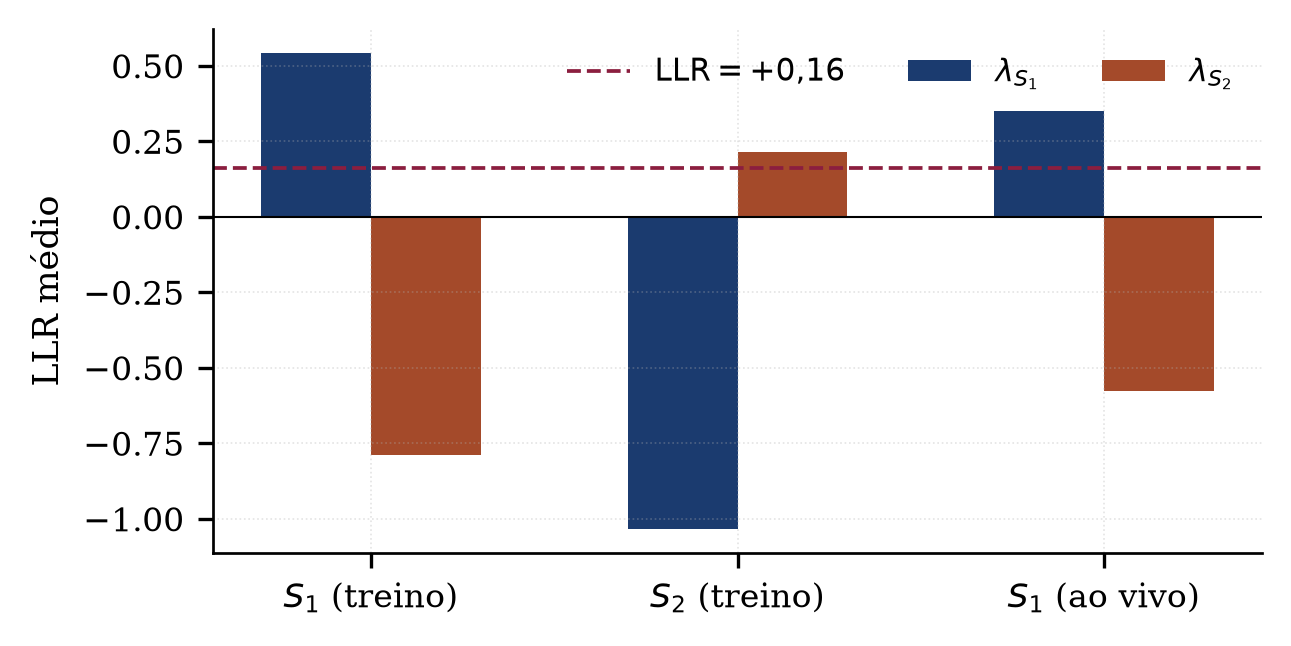
\includegraphics[width=\columnwidth]{figs/fig_gmm_llr.png}
    \caption{Pontuação LLR média por quadro obtida pelo GMM-UBM + CMN ($M=8, D=24$) nas sessões de treino e na captura ao vivo do ESP32-S3.}
    \label{fig:gmm_llr}
\end{figure}

\subsection{Avaliação em Conjunto Aberto (Open-Set: FAR, FRR e EER) e UBM Externo}
Para validar rigorosamente a rejeição de locutores desconhecidos sem vazamento de sessão nem de locutor, coletou-se uma base anonimizada de $6$ locutores masculinos no INMP441 ($19$ sessões limpas com piso $\mathrm{RMS} \le 67$, $102$ janelas de $2\text{ s}$), particionada em três conjuntos disjuntos: (i) $2$ locutores conhecidos ($S_1$ com $3$ sessões e $S_2$ com $4$ sessões, $30$ janelas ao todo, separando treino, calibração de $\tau^*$ e teste por sessão inteira); (ii) $2$ impostores exclusivos de calibração ($U_1, U_2$, $38$ janelas); e (iii) $2$ impostores inéditos de teste ($U_3, U_4$, $34$ janelas). Adicionalmente, treinou-se um \textbf{UBM externo} ($M=8, D=24$) sobre $350$ janelas ($44\,100$ quadros) do corpus público \textit{Google FLEURS PT-BR}~\cite{conneau2023}, embarcado na placa com CMN seletiva em $c_1$ e mapeamento $d_{\mathrm{eq}} = \mathrm{clip}(1 - \mathrm{LLR}/5, 0, 1)$ ($\tau = 0{,}70$, \texttt{tauver = 4}).

A Tabela~\ref{tab:openset} compara todos os modelos na média $\pm$ desvio padrão sobre $10$ partições únicas de sessão; as Figuras~\ref{fig:openset_roc} e~\ref{fig:openset_llr} exibem as curvas ROC e a separação de LLR. Os resultados justificam a adoção do \textbf{GMM-UBM (FLEURS PT-BR, Mel HTK $40$, $17$ MFCCs, $D=32$)} sob critérios tanto estatísticos quanto embarcados: (1) é o único paradigma a atingir $\mathbf{100{,}0 \pm 0{,}0\%}$ de acurácia fechada em todas as $10$ partições, o maior \textbf{AUC-ROC} ($\mathbf{95{,}5 \pm 2{,}7\%}$), o menor \textbf{EER} ($\mathbf{9{,}4 \pm 6{,}0\%}$) e a menor \textbf{FAR} ($\mathbf{6{,}8 \pm 5{,}3\%}$ --- quase $5\times$ inferior à do $k$-NN); (2) supera amplamente classificadores baseados em vetores médios (Centroide: $81{,}7\%$ AUC / $24{,}6\%$ EER; $k$-NN: $79{,}2\%$ AUC / $31{,}8\%$ EER; SVM-RBF: $69{,}1\%$ AUC / $35{,}6\%$ EER), bem como o GMM independente sem UBM ($66{,}2\%$ AUC / $40{,}7\%$ EER) e o UBM interno de $2$ locutores ($47{,}1\%$ AUC / $52{,}7\%$ EER); e (3) viabiliza cadastro ao vivo em passo único (MAP) na placa sem re-treino global (inviável em SVM/redes neurais), ocupando apenas $2{,}19\text{ KiB}$ para o UBM, $2{,}0\text{ KiB}$ para o \textit{prior} vocal em Flash e $1024\text{ B}$/locutor na NVS. Adicionalmente, em testes sob ruído aditivo de sala (ruído rosa + $60/120\text{ Hz}$ de $+15\text{ dB}$ a $+5\text{ dB}$ de SNR), a configuração com $17$ MFCCs ($D=32$) manteve $\mathrm{AUC} \ge 95{,}5\%$ e $\mathrm{EER} \le 10{,}3\%$ em todos os níveis de SNR, superando em $+25\text{ p.p.}$ de acurácia fechada a variante de $13$ coeficientes em $\mathrm{SNR} = +15\text{ dB}$.

\begin{table}[t]
\centering
\scriptsize
\setlength{\tabcolsep}{2.2pt}
\caption{Comparação entre classificadores em conjunto aberto ($6$ locutores limpos; média $\pm$ DP em $10$ splits de sessão).}
\label{tab:openset}
\begin{tabular}{lcccc}
\toprule
\textbf{Modelo} & \textbf{Acc} & \textbf{AUC-ROC $\uparrow$} & \textbf{FAR} & \textbf{EER $\downarrow$} \\
\midrule
Centroide Cosseno & $98{,}9\%$ & $81{,}7 \pm 7{,}4\%$ & $29{,}7\%$ & $24{,}6 \pm 9{,}4\%$ \\
$k$-NN Cosseno ($k{=}3$) & $97{,}8\%$ & $79{,}2 \pm 11{,}3\%$ & $28{,}5\%$ & $31{,}8 \pm 10{,}4\%$ \\
SVM (RBF) & $76{,}4\%$ & $69{,}1 \pm 14{,}6\%$ & $18{,}8\%$ & $35{,}6 \pm 14{,}7\%$ \\
GMM Indep.\ + CMN & $96{,}8\%$ & $66{,}2 \pm 8{,}8\%$ & $31{,}5\%$ & $40{,}7 \pm 12{,}8\%$ \\
GMM-UBM (UBM 2 loc.) & $96{,}7\%$ & $47{,}1 \pm 14{,}2\%$ & $47{,}6\%$ & $52{,}7 \pm 11{,}3\%$ \\
\textbf{GMM-UBM (FLEURS, CMN-$c_1$)} & $\mathbf{100\%}$ & $\mathbf{95{,}5 \pm 2{,}7\%}$ & $\mathbf{6{,}8\%}$ & $\mathbf{9{,}4 \pm 6{,}0\%}$ \\
\textbf{GMM-UBM (FLEURS, s/ CMN)} & $\mathbf{100\%}$ & $93{,}1 \pm 3{,}3\%$ & $11{,}8\%$ & $12{,}4 \pm 7{,}5\%$ \\
\bottomrule
\end{tabular}
\end{table}

\begin{figure}[t]
    \centering
    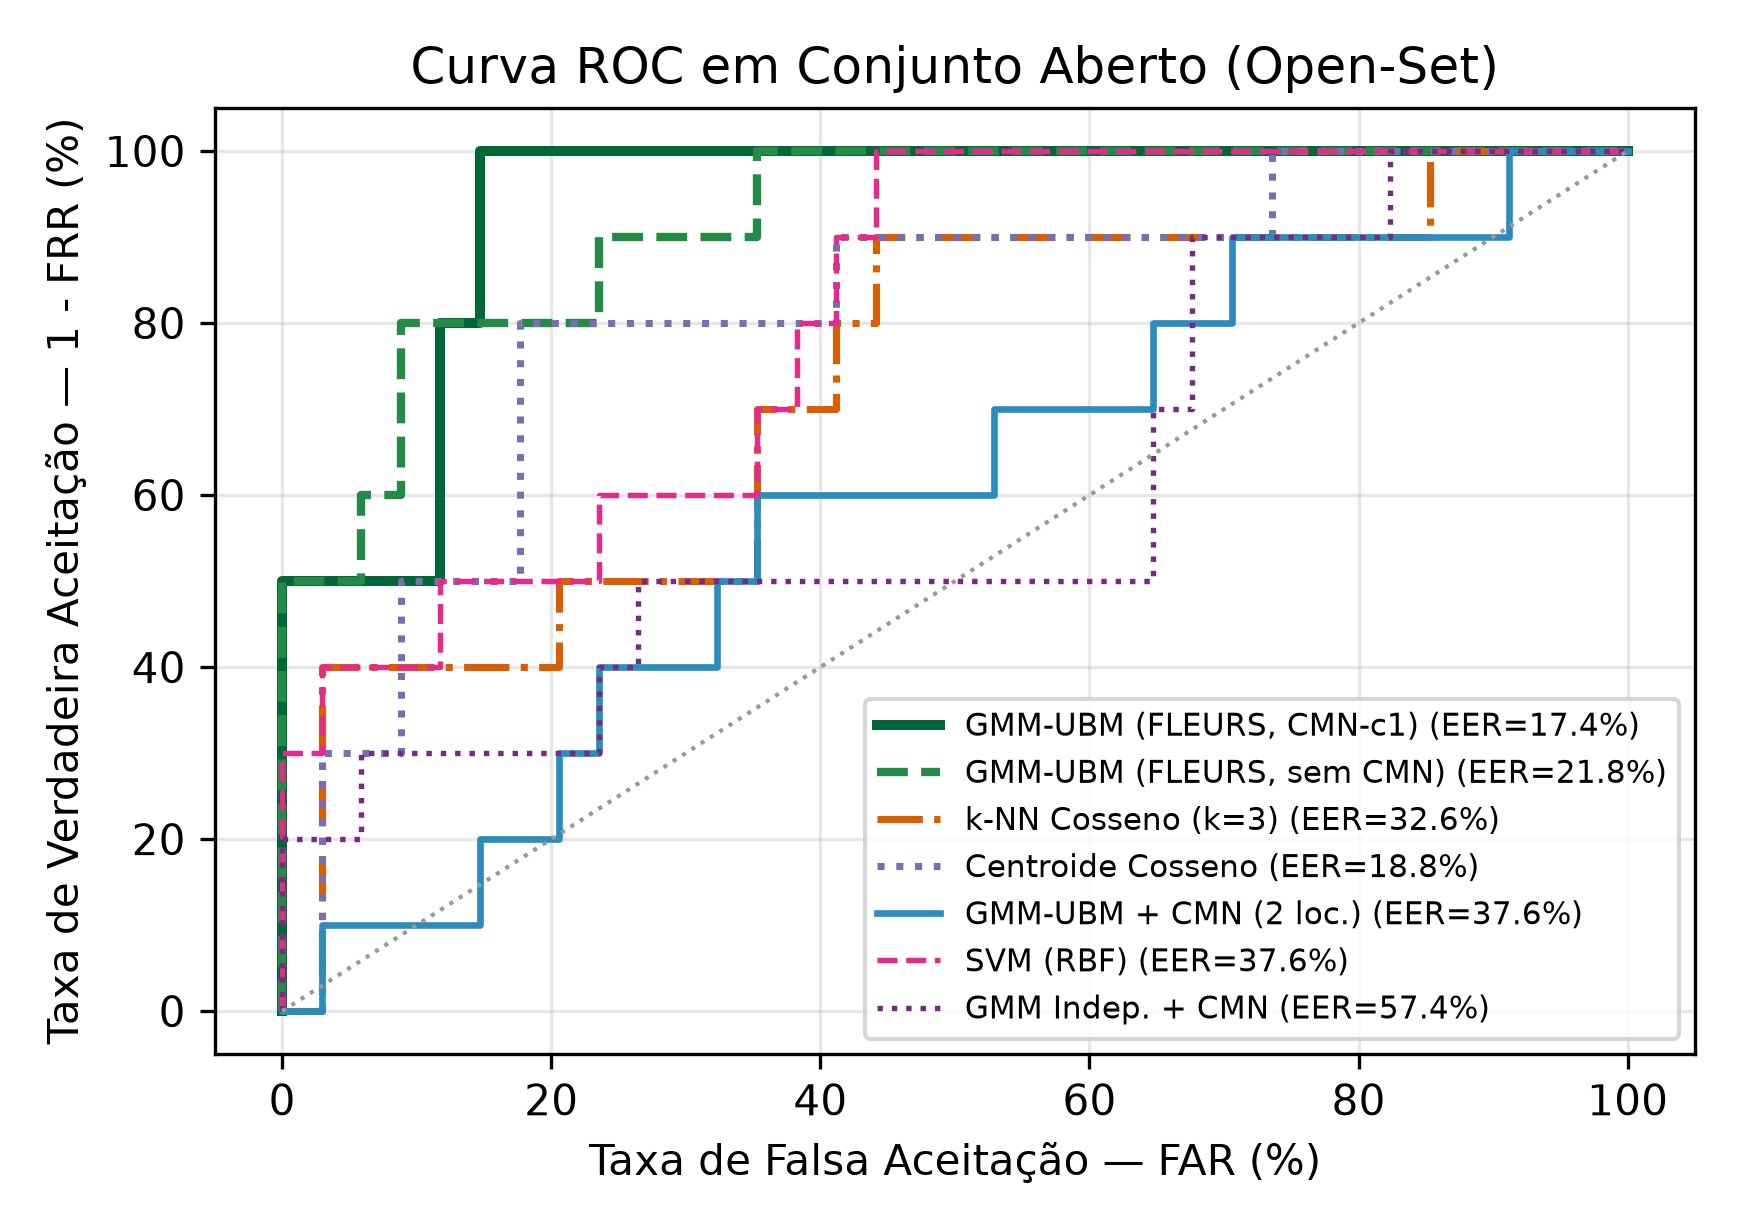
\includegraphics[width=\columnwidth]{figs/fig_openset_roc.png}
    \caption{Curvas ROC comparativas no protocolo \textit{open-set} (seed 42, $10$ janelas conhecidas vs.\ $34$ janelas de impostores inéditos $U_3, U_4$).}
    \label{fig:openset_roc}
\end{figure}

\begin{figure}[t]
    \centering
    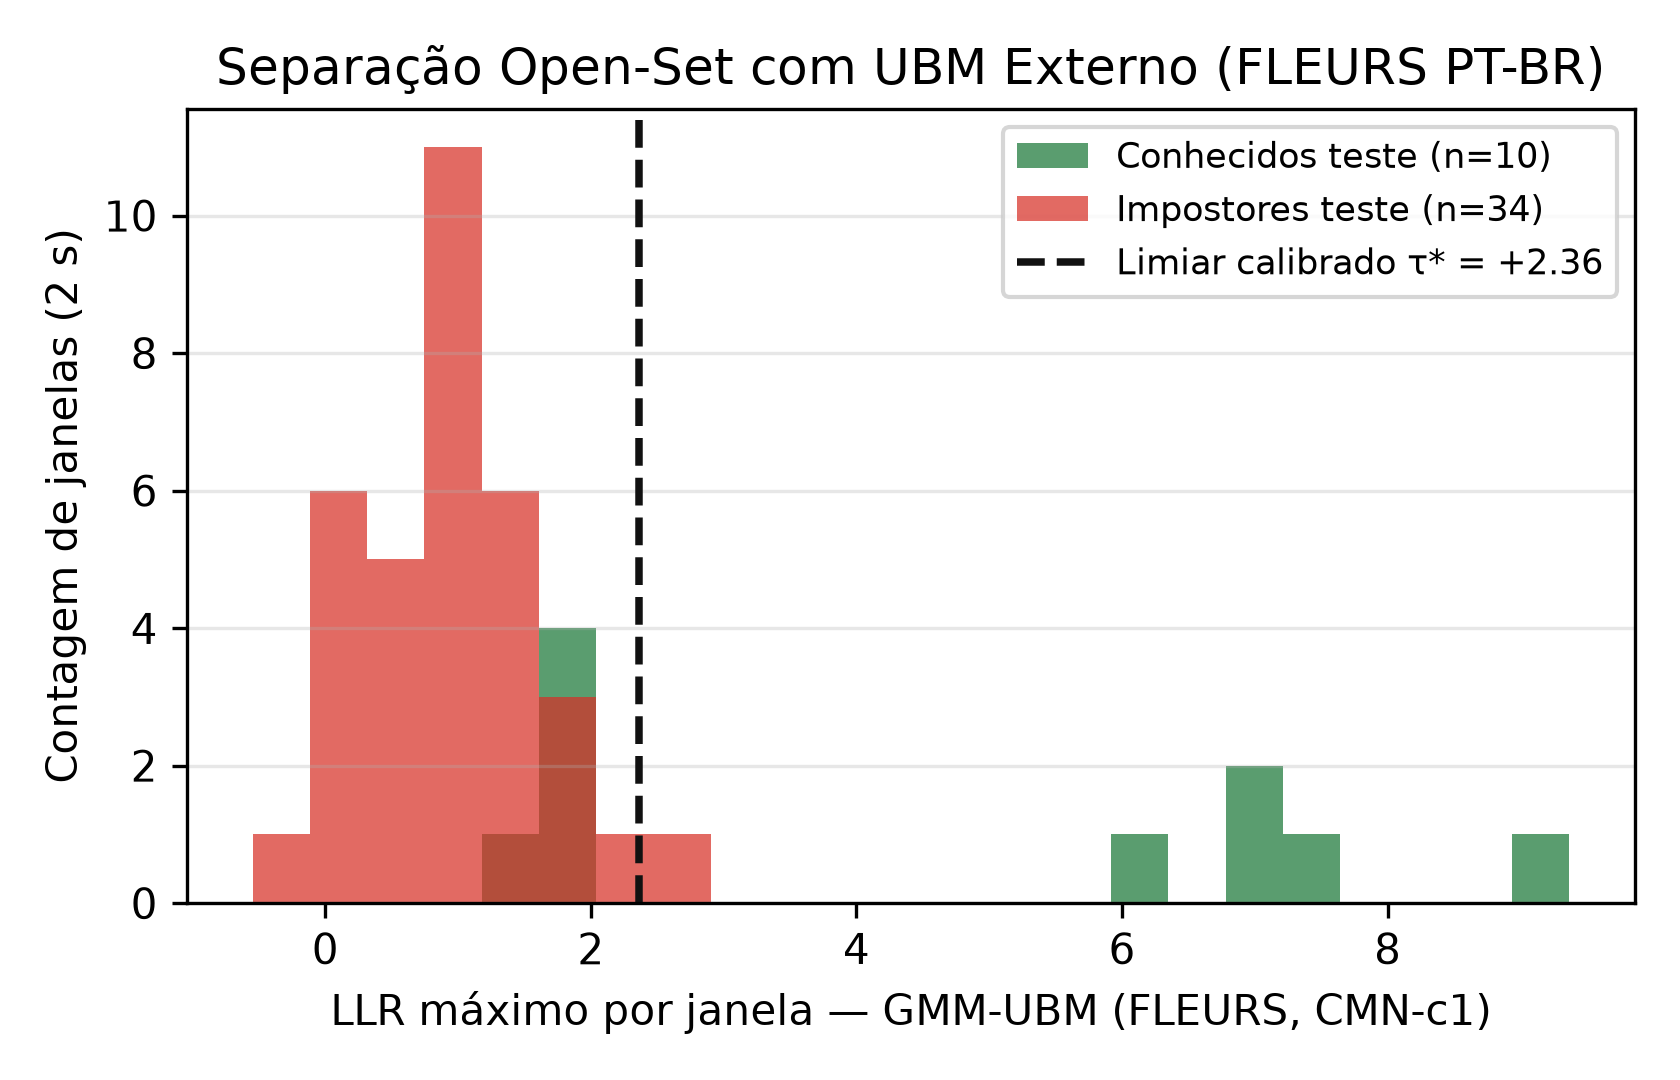
\includegraphics[width=\columnwidth]{figs/fig_openset_llr.png}
    \caption{Distribuição dos escores LLR máximos do GMM-UBM com UBM externo FLEURS PT-BR e CMN seletiva em $c_1$ ($M=8, D=24$) no conjunto de teste \textit{open-set}.}
    \label{fig:openset_llr}
\end{figure}

\subsection{Medições em Tempo Real no Hardware (ESP32-S3)}
Em testes ao vivo iniciais com ruído de sala ($\mathrm{rms} = 68$ no \textit{boot}), todas as $4$ falas consecutivas de $S_1$ ranquearam $S_1$ em $1^\text{o}$ lugar (Tabela~\ref{tab:live_esp}), atingindo margens de até $+0{,}872$ unidades de LLR sobre $S_2$. Observa-se que a fala \#3, embora tenha mantido $S_1$ à frente de $S_2$ ($\Delta\mathrm{LLR} = +0{,}140$), registrou $\mathrm{LLR}_{S_1} = -0{,}016$, ficando abaixo do limiar de aceitação ($\mathrm{LLR}_{\min} = +0{,}16$) e resultando em falsa rejeição (\texttt{DESCONHECIDO}) --- comportamento esperado sob variação pontual de prosódia ou distância em um limiar conservador.

\begin{table}[t]
\centering
\scriptsize
\setlength{\tabcolsep}{2.8pt}
\caption{Medições em tempo real no ESP32-S3 ($\tau = 0{,}420$, $\mathrm{LLR}_{\min} = +0{,}16$).}
\label{tab:live_esp}
\begin{tabular}{lccccc}
\toprule
\textbf{Cenário} & \textbf{$\mathrm{LLR}_{S_1}$} & \textbf{$\mathrm{LLR}_{S_2}$} & \textbf{$d_{\mathrm{eq}}$} & \textbf{$\mathrm{mod}$} & \textbf{Decisão} \\
\midrule
$S_1$ (\#1) & $+0{,}272$ & $-0{,}483$ & $0{,}364$ & $69{,}1$ & $S_1$ (\texttt{OK}) \\
$S_1$ (\#2) & $+0{,}168$ & $-0{,}457$ & $0{,}416$ & $58{,}8$ & $S_1$ (\texttt{OK}) \\
$S_1$ (\#3) & $-0{,}016$ & $-0{,}156$ & $0{,}508$ & $71{,}8$ & \texttt{DESC.} \\
$S_1$ (\#4) & $+0{,}261$ & $-0{,}611$ & $0{,}370$ & $71{,}1$ & $S_1$ (\texttt{OK}) \\
\midrule
$S_2$ (5 falas) & \textit{[TODO]} & \textit{[TODO]} & \textit{[TODO]} & \textit{[TODO]} & \textit{[TODO]} \\
Impostor $S_u$ & \textit{[TODO]} & \textit{[TODO]} & \textit{[TODO]} & \textit{[TODO]} & \texttt{DESC.} \\
$S_v$ (\texttt{enroll}) & \textit{[TODO]} & \textit{[TODO]} & \textit{[TODO]} & \textit{[TODO]} & $S_v$ (\texttt{OK}) \\
Ruído puro & --- & --- & --- & \textit{[TODO]} & \texttt{RUIDO} \\
\bottomrule
\end{tabular}
\end{table}

\todo[TODO 4 --- Bateria completa ao vivo no ESP32-S3 (Tabela~\ref{tab:live_esp})]{%
    Com o firmware \texttt{recvoz-esp} no monitor serial (\texttt{idf.py -p /dev/ttyACM0 monitor}):
    (1) Testar $5$ falas de $S_2$ e anotar LLR médio, $d_{\mathrm{eq}}$, $\mathrm{mod}$ e taxa de acerto.
    (2) Testar $5$ falas de pelo menos $1$ pessoa não cadastrada ($S_u$) para validar rejeição (\texttt{DESCONHECIDO}).
    (3) Executar \texttt{enroll VISITANTE} ao vivo (7 janelas), testar $5$ falas de $S_v$ (e após \texttt{reboot} para validar NVS) e registrar a LLR do modelo adaptado na placa.
    (4) Ligar ruído estacionário (ex.\ ventilador/ar) sem fala e registrar o veto \texttt{RUIDO AMBIENTE} com o valor de $\mathrm{mod}$.
}

\section{Limitações, Ameaças à Validade e Reprodutibilidade}
\label{sec:limitacoes}

Para transparência metodológica, destacam-se as seguintes limitações do protótipo atual:
\begin{description}
    \item[Tamanho da base e descasamento de microfone no UBM] Embora o UBM externo (\textit{Google FLEURS PT-BR}) com banco Mel HTK ($40$ filtros, $17$ MFCCs, $D=32$), \textit{Frame-VAD} e CMN-$c_1$ tenha obtido o maior AUC-ROC ($95{,}5 \pm 2{,}7\%$), o menor EER ($9{,}4 \pm 6{,}0\%$) e FAR de apenas $6{,}8\%$ entre os classificadores (Tabela~\ref{tab:openset}), o treino de $S_1$ com apenas $1$ sessão ($10\text{--}12\text{ s}$) e o descasamento acústico entre os microfones do corpus FLEURS e o MEMS INMP441 ainda mantêm FRR média de $24{,}3\%$ em limiar conservador. Ampliar o número de sessões de matrícula e adaptar o UBM com mais falantes no próprio INMP441 tende a reduzir ainda mais a FRR.
    \item[Sensibilidade a prosódia e distância] Como ilustrado na fala \#3 da Tabela~\ref{tab:live_esp}, variações bruscas de volume, distância ou fala sussurrada podem derrubar o LLR abaixo de $\tau$ mesmo quando o ranking relativo permanece correto.
    \item[Atomicidade da persistência NVS] Cada locutor cadastrado grava múltiplas chaves NVS (\texttt{x\%dn}, \texttt{x\%dv}, \texttt{x\%dg}). Embora o estado em RAM só seja atualizado após sucesso de escrita e \textit{commit}, uma interrupção abrupta de energia entre chaves não constitui transação atômica; versões futuras podem consolidar o cadastro em um único \textit{blob} versionado.
    \item[Reprodutibilidade] Todo o código-fonte do firmware ESP-IDF, o pacote Python, as suítes de teste no host ($7$ suítes C e $9$ testes Python executáveis via \texttt{make test}) e os scripts de avaliação (\texttt{make evaluate}) estão disponíveis publicamente em \url{https://github.com/adrianviniciuscs/recvoz}.
\end{description}

\section{Conclusão}
\label{sec:conclusao}

A substituição do $k$-NN sobre médias estáticas por um modelo probabilístico \textbf{GMM-UBM + CMN} operando quadro a quadro em $24$ dimensões ($c_1\dots c_{12} + \Delta c_1\dots \Delta c_{12}$), associada ao VAD passa-banda adaptativo, supressão espectral controlada ($\alpha = 0{,}8$) e veto por modulação articulatória, eliminou o viés acústico de cômodo e ampliou em mais de uma ordem de grandeza a separação entre locutores no ESP32-S3. A adaptação MAP de uma passada viabiliza o cadastro ao vivo de novos locutores com apenas $768\text{ bytes}$ na NVS e incremento de apenas $2{,}9\text{ KiB}$ no binário final. Trabalhos futuros incluem a expansão da avaliação \textit{open-set} com UBM treinado em corpus amplo de língua portuguesa, a consolidação atômica do formato NVS e a incorporação de frequência fundamental ($F_0$) nos quadros vozeados.

\begin{thebibliography}{9}
\bibitem{reynolds2000}
D. A. Reynolds, T. F. Quatieri, and R. B. Dunn, \enquote{Speaker verification using adapted Gaussian mixture models,} \textit{Digital Signal Processing}, vol. 10, no. 1--3, pp. 19--41, 2000.

\bibitem{reynolds1995}
D. A. Reynolds and R. C. Rose, \enquote{Robust text-independent speaker identification using Gaussian mixture speaker models,} \textit{IEEE Trans. Speech and Audio Processing}, vol. 3, no. 1, pp. 72--83, 1995.

\bibitem{loizou2013}
P. C. Loizou, \textit{Speech Enhancement: Theory and Practice}, 2nd ed. CRC Press, 2013.

\bibitem{furui1981}
S. Furui, \enquote{Cepstral analysis technique for automatic speaker verification,} \textit{IEEE Trans. Acoustics, Speech, and Signal Processing}, vol. 29, no. 2, pp. 254--272, 1981.

\bibitem{rabiner1993}
L. Rabiner and B.-H. Juang, \textit{Fundamentals of Speech Recognition}. Prentice-Hall, 1993.

\bibitem{dehak2011}
N. Dehak, P. J. Kenny, R. Dehak, P. Dumouchel, and P. Ouellet, \enquote{Front-end factor analysis for speaker verification,} \textit{IEEE Trans. Audio, Speech, and Language Processing}, vol. 19, no. 4, pp. 788--798, 2011.

\bibitem{snyder2018}
D. Snyder, D. Garcia-Romero, G. Sell, D. Povey, and S. Khudanpur, \enquote{X-vectors: Robust DNN embeddings for speaker recognition,} in \textit{Proc. IEEE ICASSP}, pp. 5329--5333, 2018.

\bibitem{desplanques2020}
B. Desplanques, J. Thienpondt, and K. Demuynck, \enquote{ECAPA-TDNN: Emphasized channel attention, propagation and aggregation in TDNN based speaker verification,} in \textit{Proc. Interspeech}, pp. 3830--3834, 2020.

\bibitem{warden2019}
P. Warden and D. Situnayake, \textit{TinyML: Machine Learning with TensorFlow Lite on Arduino and Ultra-Low-Power Microcontrollers}. O'Reilly Media, 2019.

\bibitem{conneau2023}
A. Conneau, M. Ma, S. Khanuja, Y. Zhang, V. Axelrod, S. Dalmia, J. Riesa, C. Rivera, and A. Bapna, \enquote{FLEURS: Few-shot learning evaluation of universal representations of speech,} in \textit{Proc. IEEE Spoken Language Technology Workshop (SLT)}, pp. 798--805, 2023.
\end{thebibliography}

\end{document}
